\chapter{Acceleration-Sensitive Interference}\label{chap:atom_int}

This chapter describes the work towards realising an atom interferometer and
subsequently measuring accelerations.
\section{Chapter Outline}
\verysubsection{To-Do}
\begin{itemize}
	\item Raman spectrum, identifying each transition
	\item Characterisation of velocity-selective pulse and each interferometer
	pulse using Rabi oscillations.
	\item Making a three-pulse atom interferometer
	\item Improving acceleration sensitivity and correlating vibrations using MEMS
\end{itemize}
\section{Wavefront Requirements}

\section{Raman Optical System}\label{sec:setup_ramanoptics}
When designing an optical system for the light used in an atom interferometer,
it is worth paying attention to both the spatial extent and beam waist of the
collimated beam. These requirements are particularly important in this
experiment, where acceleration due to gravity is perpendicular to the Raman beam
axis and causes significant transverse motion of the atoms. Firstly, the optical
system must be designed to make sure that the atoms are illuminated by each
interferometer pulse. In addition to this, a more subtle requirement on the
fringe contrast constrains the beam waist size. The gradient of intensity across
the atom cloud must be small so that each atom is driven by (approximately) the
same Rabi frequency. Otherwise, this variation in the Rabi frequency will
dephase the atoms, which reduces the interferometer fringe contrast.
\par\noindent A further constraint on the optical system comes from the effect
of thickness variation of optical elements. If the optical path length of the
light as it passes through an element is not uniform, this will lead to
wavefront aberrations. A spatially-varying phase leads to a bias in the
interferometer phase since it does not depend on acceleration. Moreover, since
this phase is not the same for each atom, it is another source of dephasing.
Considering the effects of wavefront aberrations was a large motivating factor
for designing an optical system for use inside the vacuum chamber. Specifically,
the distortions of a laser wavefront through optical viewports would drastically
reduce the fringe contrast under transverse motion of the atoms during the
interferometer. The process used to bond an optical viewport to a flange
stresses the glass and distorts its thickness, producing wavefront aberrations
that factor into the phase uncertainty of an atom
interferometer~\cite{Schkolnik2015}. {\huge Add requirements on other optics}
\subsection{Fringe Contrast Dependence}\label{subsec:fringe_contrast}
The effects of a gradient of intensity on the fringe contrast can be shown by
considering an ensemble of atoms that are spatially distributed by a Gaussian
distribution. Neglecting the effect of the ensemble's velocity distribution on
the Raman detuning and for fixed pulse times, the pulse area \(\Omega \tau\)
varies only as a function of the radial displacement from the optic axis. The
total fringe contrast can be determined by a convolution of the contrast for a
single atom with the atomic density
\begin{equation}
	\mathcal{C} = \int \frac{1}{\sqrt{2\pi}\sigma_c}e^{-r^2/(2\sigma_c^2)} f_{\pi/2-\pi-\pi/2}\left(\Omega(r-r_1),\Omega_(r-r_2),\Omega(r-r_3)\right) \;\mathrm{d}r
	\label{eq:cloud_contrast}
\end{equation}
where \(\sigma_c\) is the radial width of the atom cloud,
\(f_{\pi/2-\pi-\pi/2}\) is the fringe contrast as previously described in
\EquationRef{eq:fringe_contrast} and \(r_i\) is the position of the ensemble's
centre-of-mass at the \(i\)-th pulse. If the atom cloud is initially at the
centre of the laser and falling under gravity, then these coordinates are
\(\left(0, -\frac{1}{2}g T^2, -2 g T^2\right)\) respectively. Under the
assumption that the two lasers which drive the Raman transition have the same
waist size, the Rabi frequency, which is determined by the product of the
electric fields (see~\EquationRef{eg:raman_rabi}), can be described by
\begin{equation}
	\Omega(r) = \Omega_0 e^{-2 r^2/w^2}
\end{equation}
where \(\Omega_0\) is the Rabi frequency along the optic axis and \(w\) is the
waist size -- the distance at which the electric field falls to \(1/e\) of its
peak value. The fringe contrast as a function as beam waist for an atom cloud of
width a width \(\sigma_c = \sivalue{5}{\milli\metre}\) and a time between
interferometer pulses of \(T = \sivalue{25}{\milli\second}\) is plotted in
\FigureRef{fig:raman_fringecontrast}. For small beam waists, the intensity
gradient across the cloud significantly reduces the fringe contrast. In fact, a
beam waist much greater than the width of the cloud is necessary to achieve a
large contrast between the two interferometer states. Relaxing the assumptions
made on the ensemble's velocity distribution to include its influence on the
detuning and spatial distribution of the atoms during the interferometer would
strengthen this argument.
\begin{figure}[!htbp][!ht]
	\centering
	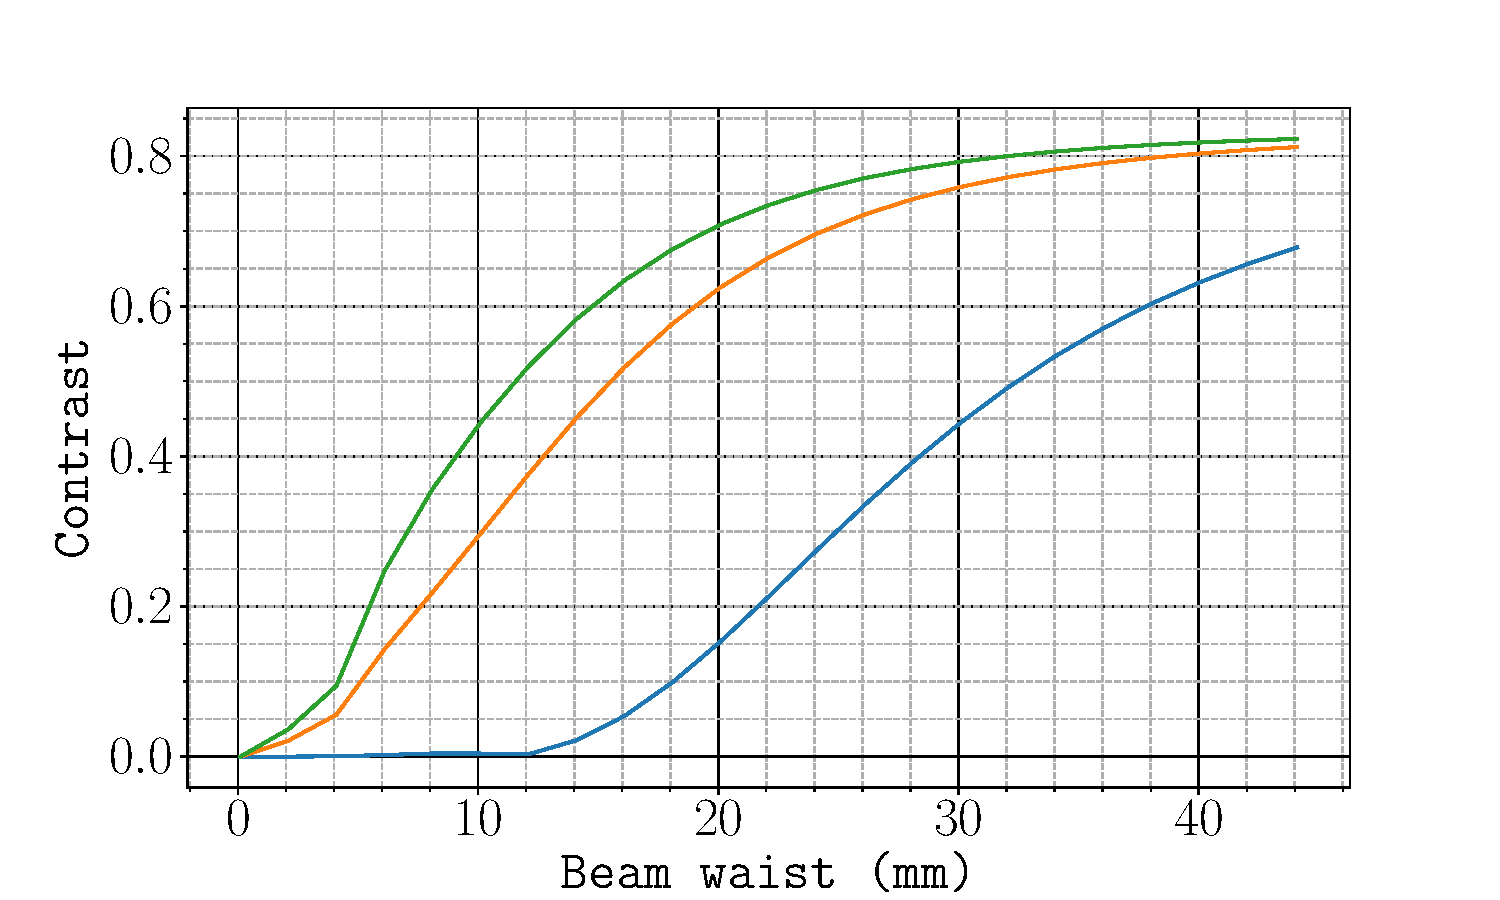
\includegraphics[width=0.5\textwidth]{fringe_contrast.pdf}
	\caption[Simulated fringe contrast vs beam waist size]{Simulated fringe
		contrast as a function of waist size \(w\) for an atom cloud falling under
		gravity. This model assumes a Gaussian distributed atomic density with a
		width \(\sigma_c = \sivalue{5}{\milli\metre}\) and a time between
		interferometer pulses of \(T = \sivalue{25}{\milli\second}\). For smaller
		beam waists the subsequent interferometer pulses have a larger intensity
		gradient across the atom ensemble, which increases the dephasing of the two
		states and reduces the interferometer fringe contrast.}
	\label{fig:raman_fringecontrast}
\end{figure}

So far, it has been shown that a large beam waist is necessary to achieve a high
fringe contrast when allowing for transverse motion of the atoms across the
laser wavefront. Otherwise, if the fringe contrast was poor, this would limit
the sensitivity of the interferometer to accelerations rather than other effects
which are less rectifiable. Another optical effect which influences the
sensitivity is distortions of the laser wavefront. In an ideal case, the
superposition of the spherical wavefronts of the two lasers results in a planar
wavefront for the effective field which drives the Raman transition. However,
propagation through rough optical elements distort these wavefronts and
introduce a spatially varying component of the Raman phase that is independent
of acceleration. If the atom cloud's trajectory is parallel with the Raman axis,
then this additional phase is the same at each laser pulse and is therefore
cancelled out. Of course, this does not occur when the cloud moves transverse to
the Raman axis where this random phase has the effect of reducing the fringe
contrast. Starting with the assumption that this phase is Gaussian distributed
around 0, with a standard deviation of \(\sigma_\phi\), if this is uncorrelated
at each interferometer pulse, then the interferometer phase \(\Delta \Phi\) will
be distributed with a standard deviation of \(\sigma_\Phi = \sqrt{6}
\sigma_\phi\). Denoting this random phase as \(\delta\phi\), the fringe contrast
is then given by
\begin{equation}
	\mathcal{C}(\delta \phi) = \cos\left(2 \delta\phi\right)
\end{equation}
Following from this, if \( \delta \phi\) is uncorrelated between each atom, the
expected value of the contrast over the ensemble is given by
\begin{align}
	\langle \mathcal{C} \rangle & = \frac{1}{\sqrt{2\pi}\sigma_\Phi}\int \mathcal{C}(\delta \phi) \; e^{-\delta\phi^2/2\sigma_\Phi^2} \; \mathrm{d}\delta\phi \\
	                            & = e^{-2 \sigma_\Phi^2}
\end{align}
The value of this expected contrast is plotted in
\FigureRef{fig:raman_phasenoise} and shows a strong dependence on
\(\sigma_\phi\). {\huge Add more justification here. Cite Achim Peter's paper}
\begin{figure}[!htbp]
	\centering
	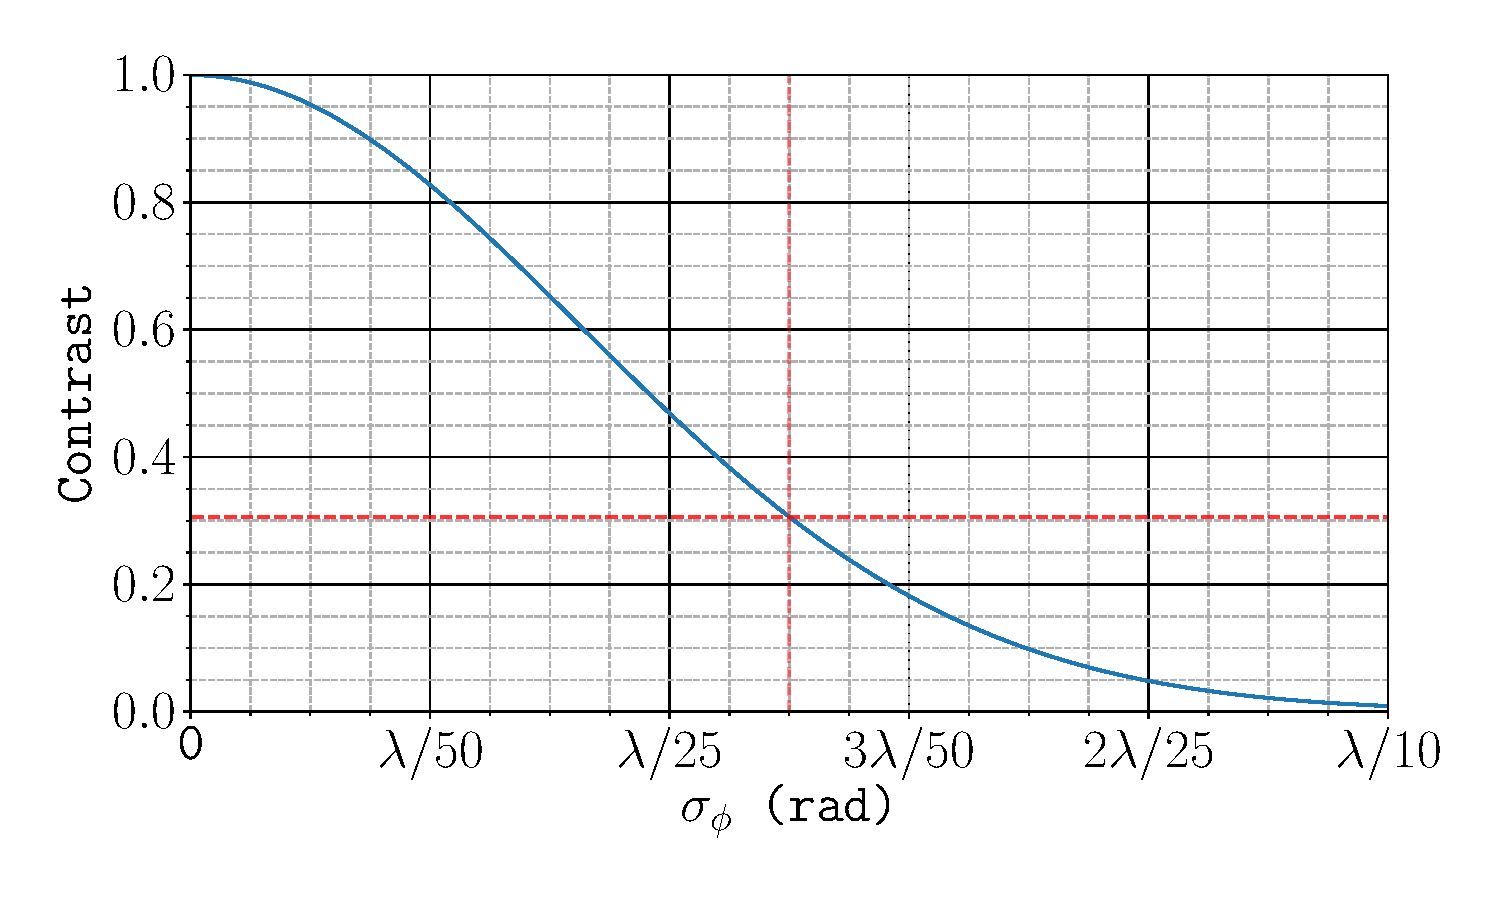
\includegraphics[width=0.5\textwidth]{phase_noise_contrast.pdf}
	\caption{Expected contrast as a function of random phase contributions. This
		assumes that the phase imprinted on an atom during each interferometer pulse
		has an additional random component that is Gaussian distributed around 0
		with a standard deviation of \(\sigma_\phi\). This random phase is also
		uncorrelated between each pulse so that the total can be obtained using
		Gaussian propagation of error. The dashed lines indicate the contrast for
		phase noise expected from conventional optics, which are usually engineered
		to a surface flatness of \(\lambda/20\).}
	\label{fig:raman_phasenoise}
\end{figure}
\subsection{Raman Beam Collimator}\label{subsec:setup_ramancollimator}
The optical system used to produce the beams for driving Raman transitions,
which will conventionally be referred to as the Raman optics, was designed to
reduce the previously mentioned effects which result in poorer interferometric
fringe visibility and sensitivity to accelerations. Principally, the entire
optical system was mounted inside the optical chamber so that the Raman light
does not pass through any optical viewports before interacting with the atoms.
Typically, the stress placed on the glass during the bonding process will
distort the flatness more than is acceptable for achieving a high contrast. For
example the viewports used for the \ac{mot} optics have a specified flatness of
\(\lambda/4\), so mounting the entire optical system inside the chamber was the
simplest way to avoid a large distortion. \par\noindent
\FigureRef{fig:raman_collimator} presents a diagram of the components used to
send Raman light into the chamber and produce a collimated beam in the centre of
the chamber. The light is coupled into the chamber using a UHV compatible
\ac{pm} fibre, manufactured by Diamond photonics. This is a kapton-coated PM-780
HP fibre that is bonded on one end to a DN16 flange using an epoxy resin. The
external side of this flange has an FC/APC connector for coupling light from
another fibre. Inside the chamber, the ferrule is connected to an FC/APC fibre
plate. This is clamped between a piece which bolts onto the inside of a DN63
flange and another stainless steel plate which bolts onto the rest of the optics
assembly. Fine adjustment of the position of the fibre along the optic axis is
achieved using shim plates with a thickness ranging from
200--\sivalue{300}{\micro\metre}. The fibre plate is free to rotate so that the
orientation of the fibre with respect to a \ac{qwp} at the output of the
collimator. This \ac{qwp} is manufactured by Light Machinery, and is described
further is \SectionRef{subsec:setup_ramanmirror}. When the fibre is correctly
orientated (e.g. when the slow axis of the fibre is at 45\(\deg\) to the slow
axis of the waveplate), the two Raman light fields are orthogonally circularly
polarised. \par\noindent The original design for the optical system consisted of
a triplet lens, as a system of three lenses is capable of correcting for the
five types of Seidel aberrations that distort rays of monochromatic light. This
was designed and manufactured by IC Optical Systems. Another specification for
this lens system was that it had to produce a collimated beam with a waist size
of around \sivalue{35}{\milli\metre} so that the sensitivity of the
interferometer was not limited by the effects of intensity gradients across the
atoms. Unfortunately, the triplet was designed with an incorrect \ac{na}. With a
focal length of \sivalue{123.4}{\milli\metre} and a diameter of
\sivalue{50}{\milli\metre}, the triplet lens has a \ac{na} of 0.194. However,
the nominal \ac{na} for PM780-HP fibre used in the UHV compatible \ac{pm} fibre
is 0.12. Consequently, the light from this fibre did not fill the \ac{na} of the
triplet lens and produced a beam with a waist of 13mm. {\huge Plot to illustrate
this}. To address this issue, a pair of aspheric lenses was included to increase
the divergence angle of light from the fibre. These are manufactured by Thorlabs
and have a focal length of \sivalue{4.51}{\milli\metre} (352230-B) and
\(\sivalue{15.29}{\milli\metre}\) (352260-B), respectively, to give a
magnification of 3.39.
\begin{figure}[!htbp]
	\centering
	\def\svgwidth{\columnwidth}
	\subfloat[][]{\scalebox{0.4}{\input{Figures/Chapter6/raman_optics.pdf_tex}\label{fig:raman_collimator}}}
	\subfloat[][]{\scalebox{0.4}{\input{Figures/Chapter6/mirror_mount.pdf_tex}\label{fig:mirror_mount}}}
	\caption[Drawings of the compenets used in the Raman optics
		assemblies]{Diagrams of the componets used in the Raman optical assemblies.
		(a) shows the collimator setup. Light is coupled into the chamber using a
		UHV fibre feedthrough. A pair of aspheric lenses is used to increase the
		divergence angle of the fibre output, before the light is collimated by a
		triplet lens. Finally, a quarter-wave plate is aligned so that it circularly
		polarises the collimated light fields. (b) illustrates the other half of the
		setup, which is used to retro-reflect the light. A second quarter-wave plate
		is used so that the reflected beams have the same handedness to their
		respected incoming ones. A MEMS accelerometer is mounted on the back of the
		mirror to measure vibrations. These components are all mounted on a
		piezo-controlled mirror mount whose tilt can be controlled from outside the
		vacuum chamber.}
	\label{fig:raman_optics}
\end{figure}
\subsubsection{Alignment and Collimation}
As one of the main motivations for mounting the Raman optics inside the vaccuum
chamber was to reduce the effects of wavefront distortions, it is worth
highlighting how inaccurate alignment of the optics can lead to aberrations. As
discussed before (see \SectionRef{subsec:fringe_contrast}), distortions of the
wavefront leads to a dephasing and loss of interferometer fringe visibility.
Here, the same figures of merit as before are used to consider what misalignment
is acceptable to ensure that the phase of the Raman wavefront deviates by less
than \(\lambda/100\) after a transverse distance of
\sivalue{12.5}{\milli\metre}. \par\noindent Taking the fibre as a point source,
misalignment can occur if it is displaced from the front focal point of the
optical system longitudinally along or transversely to the optic axis. If it is
transversely displaced, this manifests as an angular displacement of the
collimated light after the triplet lens. A large angular displacement is
undesirable due to the fact that since one of the Raman light fields propagates
further, the two wavefronts that drive acceleration-sensitive Raman transitions
are not parallel. \FigureRef{fig:raman_wave_transverse} shows a simulation of
the wavefront distortion as a result of this transverse misalignment. This is
obtained by simulating the propagation of rays corresponding to each Raman light
field through the optical system. The wavefront is estimated using the slope of
each ray at a distance of \sivalue{43}{\milli\metre} from the output of the
triplet lens, which corresponds to the position of the centre of the vacuum
chamber. The mirror is mounted at the same distance from the centre, so the
second beam propagates \sivalue{129}{\milli\metre}. Close to the optic axis,
this distortion is approximately linear (i.e. a tilt) and it can be seen that a
displacement of the fibre from the optic axis of <\sivalue{1}{\milli\metre} is
sufficient to achieve the desired wavefront flatness. \par\noindent Aside from a
transverse displacement, it is possible that the fibre could be misaligned along
the optic axis. In which case, the output beam will not be collimated.
Consequently, the counter-propagating reflected rays will not be antiparallel to
incoming ones. The effect of this longitudinal displacement on the Raman
wavefront is shown in~\FigureRef{fig:raman_wave_longitudinal}. Further from the
optic axis the deviation in the phase of the light is greater, giving a
quadratic distortion which is characteristic of a defocus. Comparing the
wavefront distortion in this case, a requirement on the longitudinal
misalignment of \(< \sivalue{0.6}{\milli\metre}\) is needed for the previously
specified flatness.

\begin{figure}[!htbp]
	\centering
	\def\svgwidth{\columnwidth}
	\subfloat[][]{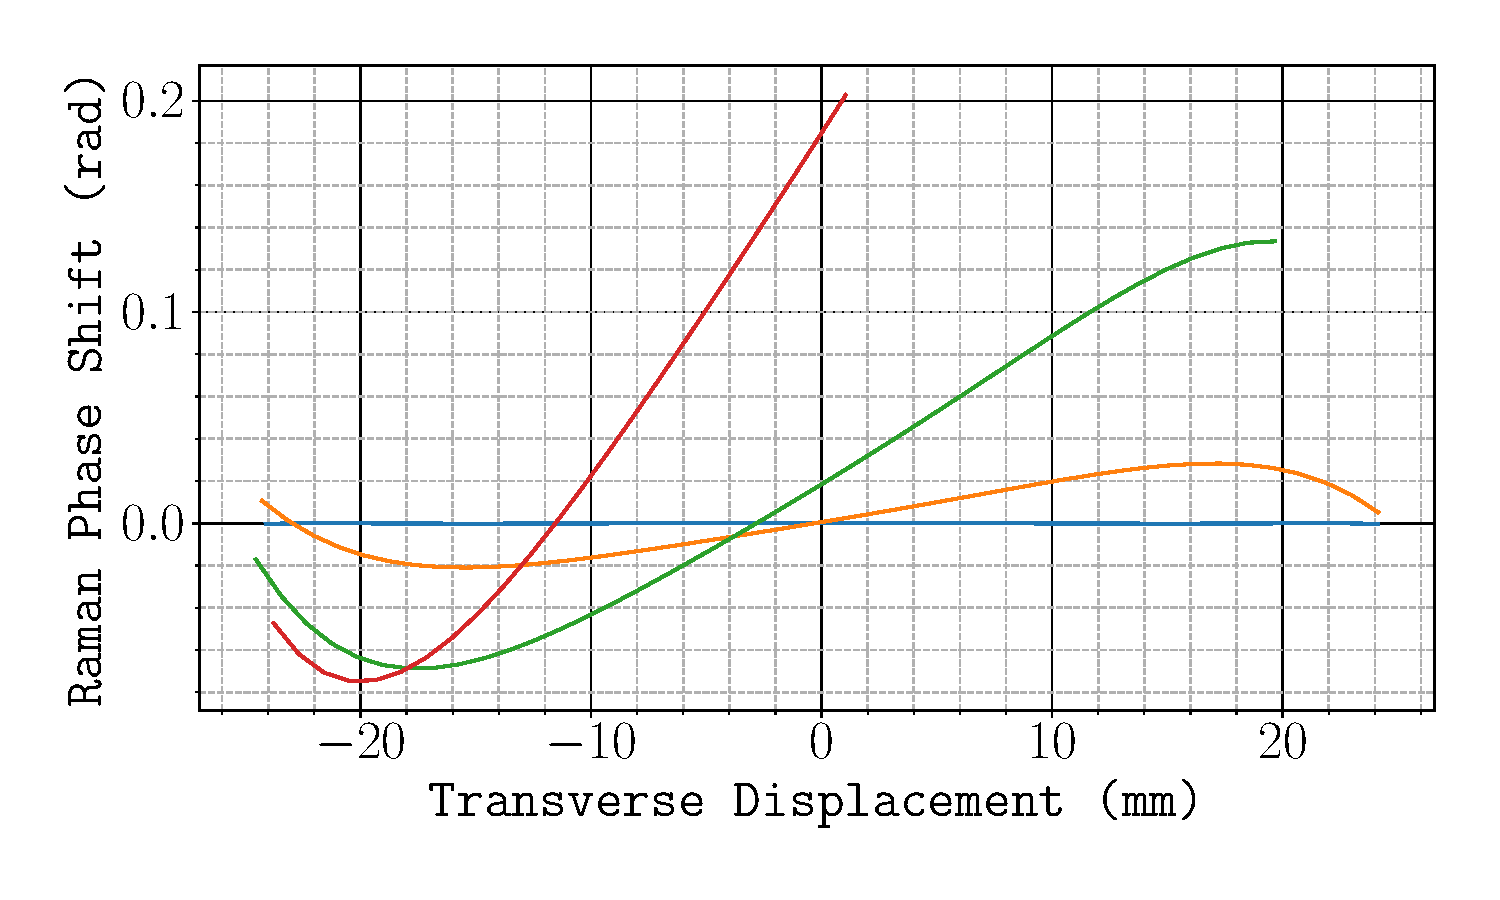
\includegraphics[width=0.4\textwidth]{wavefront_transverse.pdf}\label{fig:raman_wave_transverse}}
	\subfloat[][]{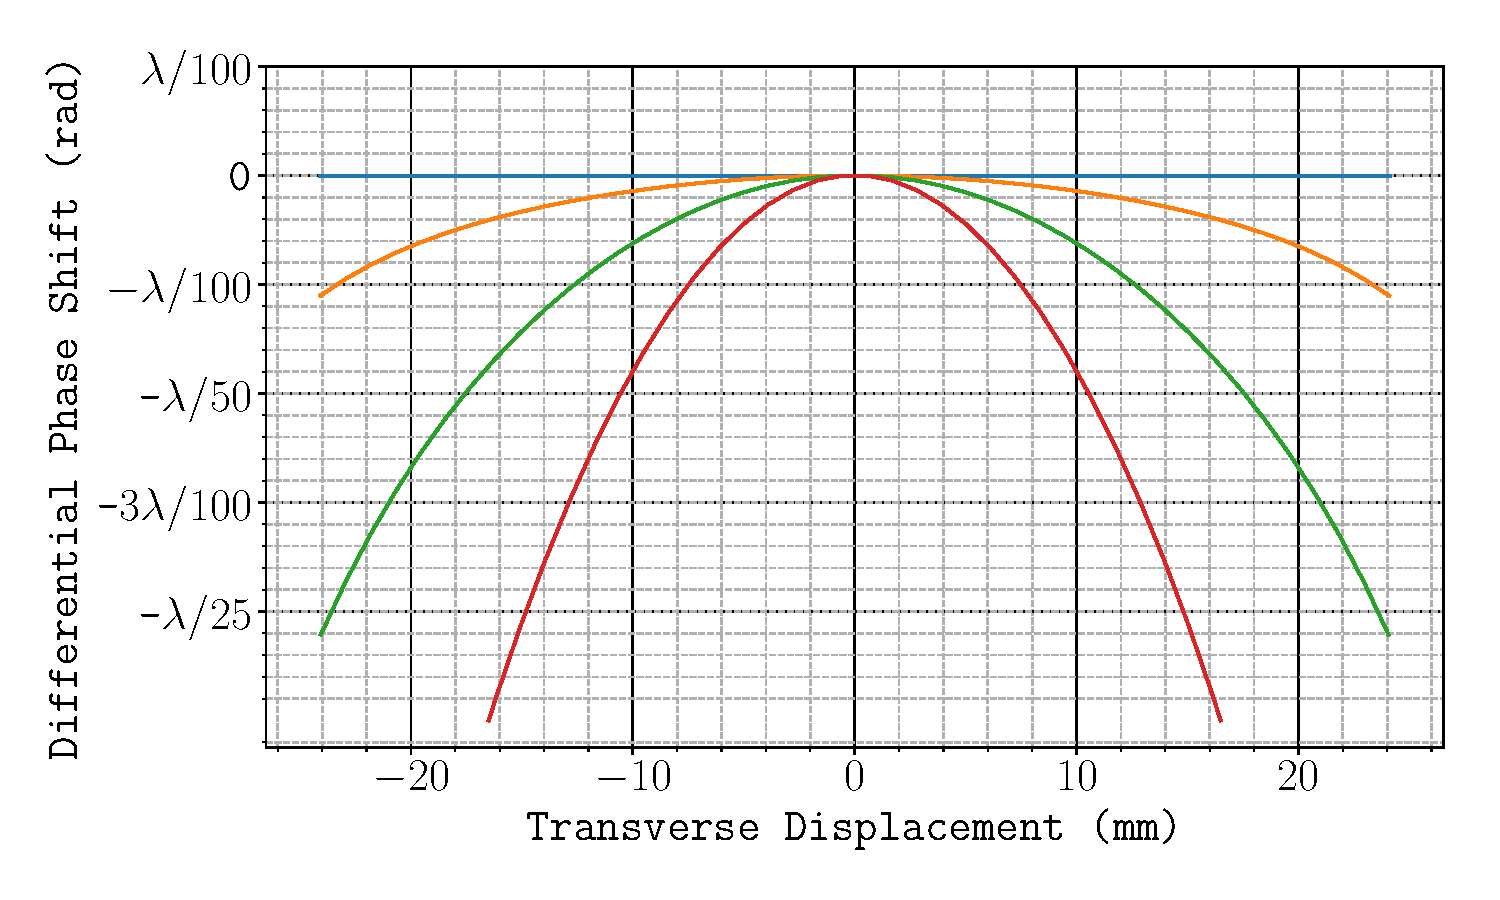
\includegraphics[width=0.4\textwidth]{wavefront_longitudinal.pdf}\label{fig:raman_wave_longitudinal}}
	\caption[Simulated wavefront distortion for longitudinal and transverse fibre
		misalignment]{Simulated wavefront distortion for longitudinal and transverse
		fibre misalignment. Rays from a point source with a divergence angle
		corresponding to a \ac{na} of 0.12 are propagated through the Raman optical
		system. Rays corresponding to the reflected beam are propagated further with
		the assumption that the mirror is perpendicular to the optic axis. The first
		set of rays propagates \sivalue{43}{\milli\metre} and the second propagates
		\sivalue{129}{\milli\metre}. The wavefront for each beam is calculated by
		taking the slope of each ray and subtracting from the slope of the central
		ray. The wavefront of the effective field that drives the Raman transition
		is the difference of these two wavefronts. (a) shows the distortion of the
		wavefront for a transverse misalignment of the fibre for a displacement of
		\sivalue{0}{\milli\metre} (blue), \sivalue{0.5}{\milli\metre} (orange)
		\sivalue{1}{\milli\metre} (green) and \sivalue{1.5}{\milli\metre} (red) from
		the front focal point. (b) shows the wavefront for longitudinal
		displacements of \sivalue{0}{\milli\metre} (blue),
		\sivalue{0.3}{\milli\metre} (orange)
		\sivalue{0.6}{\milli\metre} (green) and \sivalue{1}{\milli\metre}
		(red).}\label{fig:fig_label}
\end{figure}
\subsubsection{Measuring the Beam Width}
To measure the waist of the beam, its reflection from a flat surface was imaged
using a CCD camera. The radius of the triplet lens is smaller than the beam
waist, so the beam is apertured by this lens. To take account of this aperture,
the beam waist was estimated using a Taylor expansion of a Gaussian to second
order:
\begin{align}
	I(x) & = A e^{-\frac{(x-x_0)^2}{2 w^2}} \nonumber                                                                              \\
	     & \approx A-\frac{2 A x_0^2}{w^2}+\frac{4 A x x_0}{w^2}-\frac{2 A x^2}{w^2} + \mathcal{O}(x^3) \label{eq:gaussian_approx}
\end{align}
A typical intensity profile along the hoirzontal and vertical camera axes is
shown in~\FigureRef{fig:beam_examp}. A threshold intensity value excludes
contributions from pixels outside of the spatial extent of the beam. The waist
was estimated using a linear least-squares fit of the intensity profile to a
second-order polynomial \(c_0 + c_1 x + c_2 x^2\), where \begin{equation} w =
\left|\frac{\sqrt{c_1^2-4c_0 c_2}}{\sqrt{2}c_2} \right| \end{equation} A plot of
the estimated beam waist over a propagation distance of \sivalue{1}{\metre} is
shown in~\FigureRef{fig:beam_waist}. Inside the chamber each Raman beam
propagates \sivalue{5.25}{\centi\metre} and \sivalue{15.75}{\centi\metre}, where
the beam is well collimated. Along the vertical axis, the beam has a waist of
around \sivalue{36.9}{\milli\metre}. The horizontal waist is smaller because the
camera was horizontally tilted from the beam's optic axis. The projection of the
beam onto this axis is consistent with a horizontal tilt of
\sivalue{16}{\degree}.  \begin{figure} \centering
	\def\svgwidth{\columnwidth}
	\subfloat[][]{\scalebox{0.3}{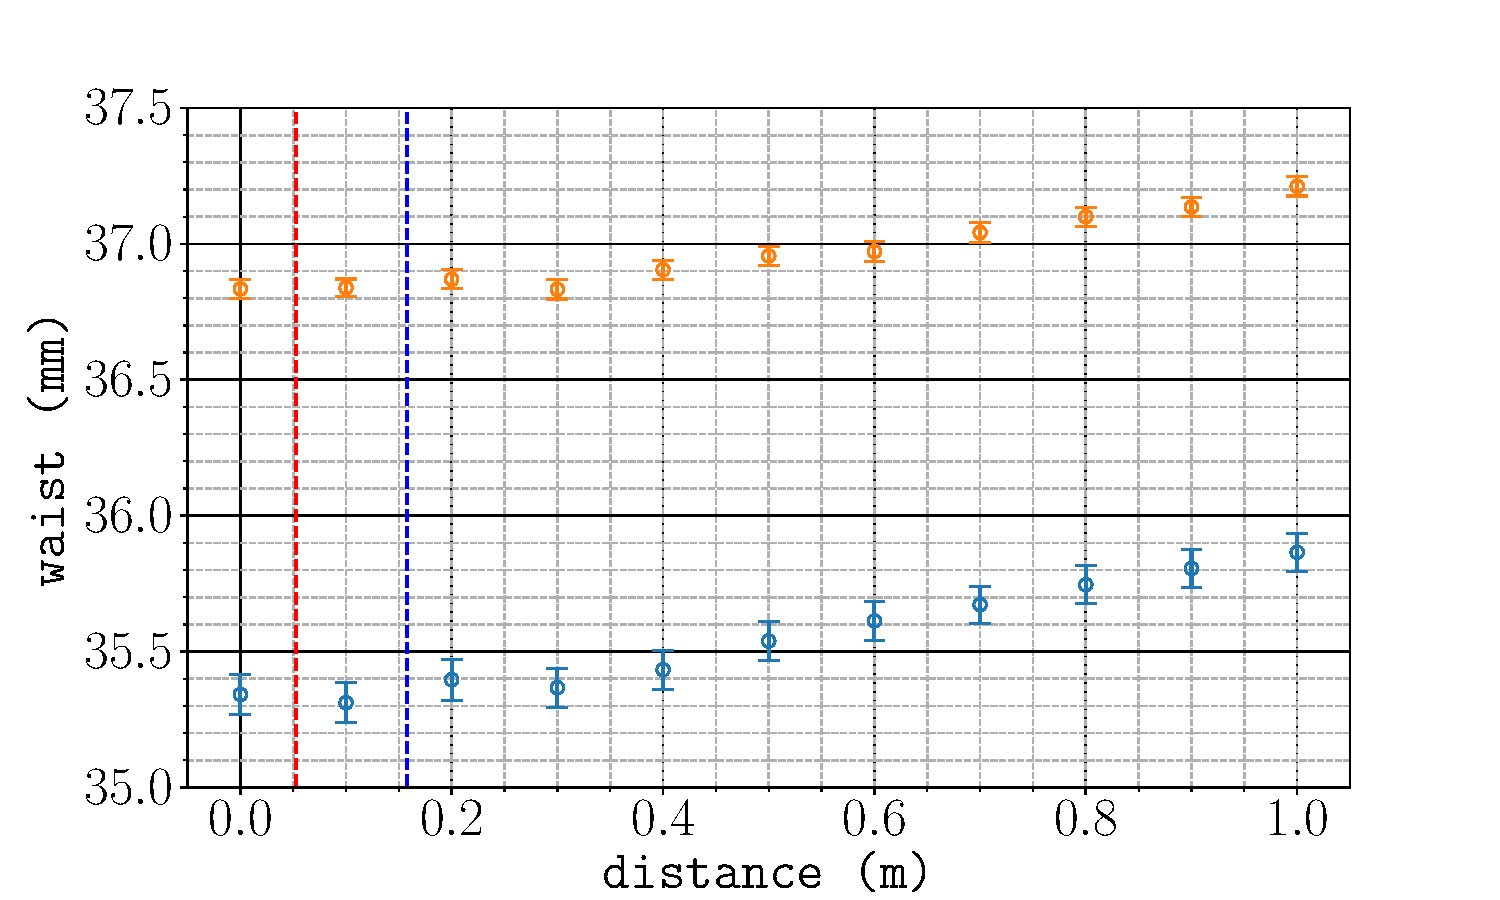
\includegraphics{beam_waist}}\label{fig:beam_waist}}
	\subfloat[][]{\scalebox{0.3}{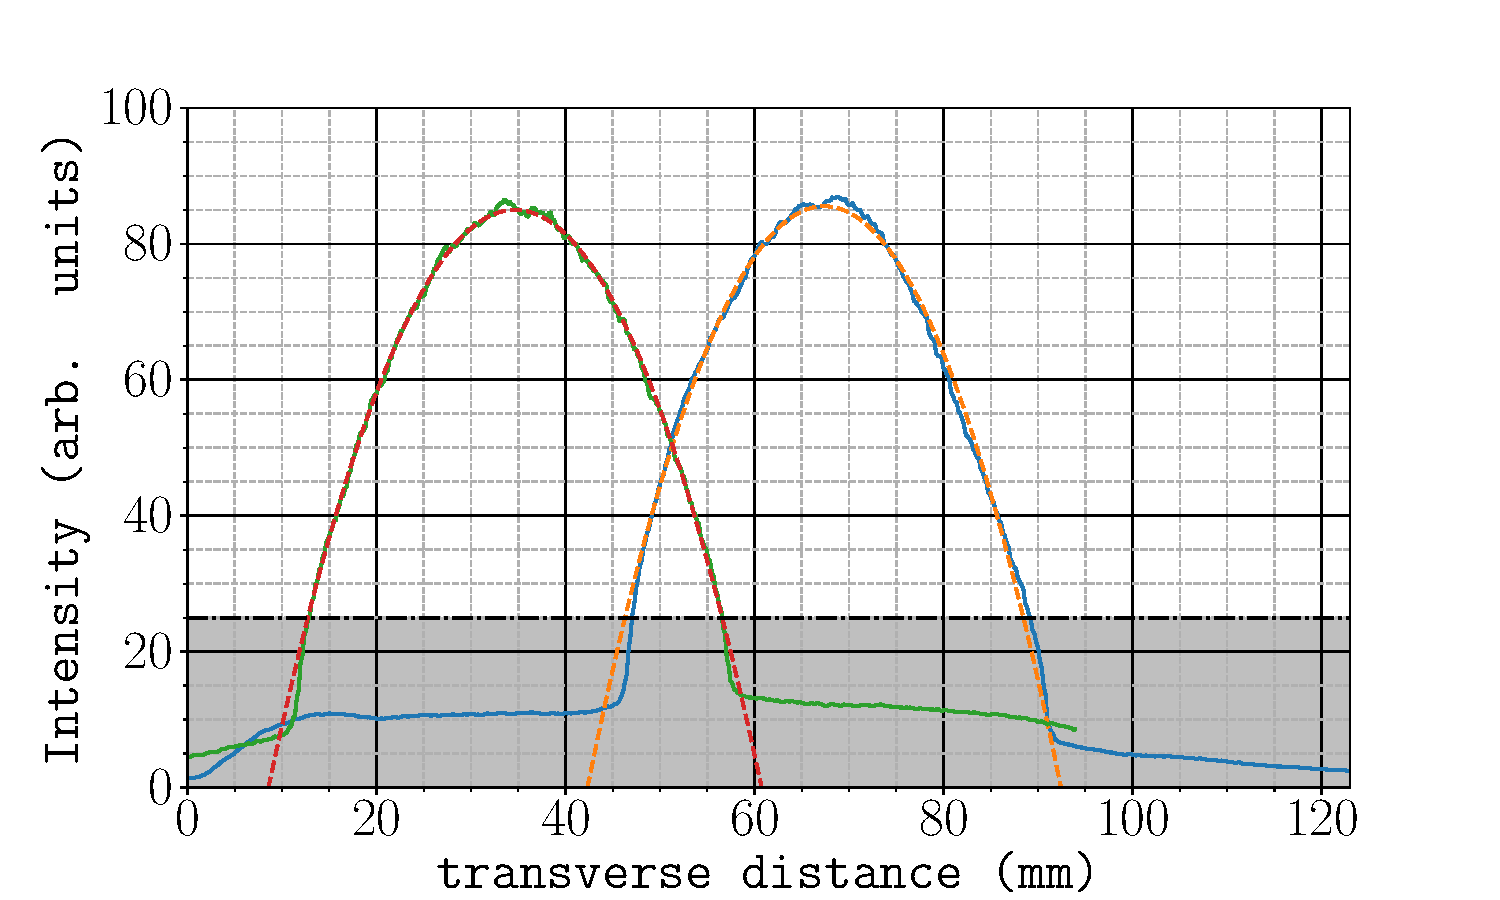
\includegraphics{beam_examp}}\label{fig:beam_examp}}
	\caption[Measured Raman beam waist]{Raman beam waist measured over a distance
		of \sivalue{1}{\metre}, shown in \textbf{(a)}. The waist along the
		horizontal and vertical axes are indicated in blue and orange respectively.
		The dashed lines indicate the approximate propagation distance of each beam
		at the position of the atoms. \textbf{(b)} shows the intensity profile along
		each axis, with the fitted parabola. The dot-dashed line is a threshold
		intensity value, which excludes pixels from outside the spatial extent of
		the beam.} \label{fig:beam_waist_plots} \end{figure}
		\subsection{Retro-reflection Assembly}\label{subsec:setup_ramanmirror} The
		Raman transitions used in the interferometer are driven by
		counter-propagating light fields to give a large momentum transfer of \(2
		\hbar k\) to the atoms. The two beams enter from the same fibre input, so a
		mirror is used to retro-reflect them. The retro-reflection assembly includes
		a \ac{qwp} to ensure that the reflected beams have the same polarisation
		handedness as their circularly polarised incoming counterpart. \par\noindent
		The mirror is also manufactured by Light Machinery, and the \ac{qwp} is made
		to the same specifications as the one that circularly polarises the incoming
		beams.  During the manufacturing process, the waveplates and mirror were
		polished to reduce irregularities in the thickness of each \ac{qwp} and the
		surface of the mirror. \FigureRef{fig:waveplate_map} shows the variation in
		the thickness of the waveplate in front of the triplet lens, measured by
		Light Machinery using a white light interferometer. This has a standard
		deviation of \sivalue{4.62}{\nano\metre} and corresponds a standard
		deviation of the optical path length of \pow{8.6}{-3}\(\lambda\).
		\begin{figure}[!htbp] \centering
	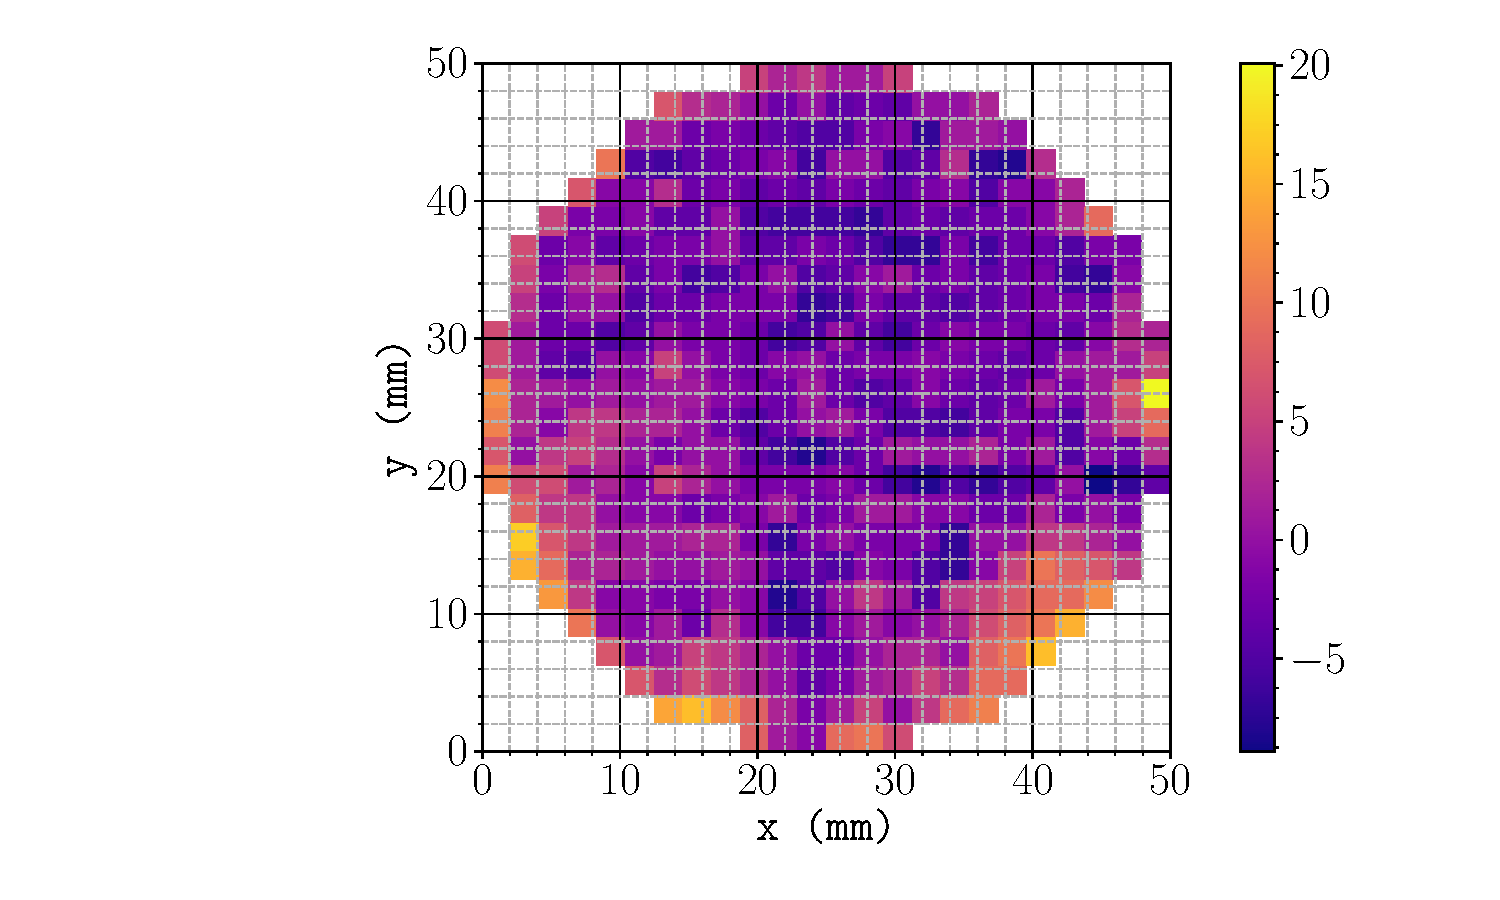
\includegraphics[width=0.5\textwidth]{waveplate.pdf}
	\caption{Thickness of the first \ac{QWP}, measured by a white light
		interferometer. The value is given in \sivalue{}{\nano\metre} as a
		difference from the mean thickness. The standard deviation of this thickness
		is \sivalue{4.62}{\nano\metre} and a peak-to-valley (PV) of {\textbf need
		number here}. Equivalent surface data for the other \ac{QWP} and mirror were
		not provided by Light Machinery, but had a PV thickness variation of
		\sivalue{19}{\nano\metre} and
		\sivalue{9}{\nano\metre} respectively.} \label{fig:waveplate_map}
\end{figure} \par\noindent The \ac{qwp} and mirror are fixed onto the front
plate of a UHV compatible MDI-HS mirror mount, manufactured by Radiant dye. The
horizontal and vertical tilt of the mirror can be adjusted using two thumbscrew
actuators which cause the front plate to pivot around a ball bearing. This mount
is designed for high stability, but of course the alignment will still drift
over time. To avoid the need to periodically open the chamber to realign the
mirror, a piezo-electric stack is placed between each actuator and the front
plate so that the tilt of the mirror can be adjusted externally. Each
piezo-stack is connected to a high-voltage feedthrough, so that their length
(and hence mirror tilt) can be finely adjusted by controlling the voltage
applied across them. A control voltage ranging between 0--\sivalue{10}{\volt} is
amplified by a controller to give an applied voltage across the piezo stack
between -10--\sivalue{150}{\volt}. This corresponds to a travel range of
\sivalue{23}{\micro\metre}. \par\noindent To understand the effect of
misalignment, it is instructive to consider its effect on the effective
wavevector \(\keff\). As illustrated in \FigureRef{fig:retro_misalign}, if the
mirror is misaligned from the incoming beam's wavevector by an angle \(theta\),
the two counter-propagating fields that drive Raman transitions have wavevectors
\(k_1 \left(1,0\right)\) and \(k_2 \left(\cos(\theta),\sin(\theta)\right)\).
\(\keff = {\textbf k_1} - {\textbf k_2} \cos (2\theta_i)\). Fortunately, for
small angular displacements, i.e. \(< \sivalue{1}{\milli\radian}\), this does
not greatly reduce the sensitivity to accelerations. In short, this means that
\(\keff\) will have a spatially varying direction. Since an atom interacting via
a Raman transition picks up a phase \(\phi = \keff . {\textbf x}\), atoms
travelling along different trajectories will accumulate different phases due to
the spatial variation of \(\keff{}\). Across the atom ensemble, this leads to a
dephasing and consequently, a loss of interferometer fringe
visibility~\cite{Tackmann2012} \subsubsection{In-Situ Alignment and
Optimisation} After mounting the Raman optical system inside the chamber, the
mirror had to be aligned to retro-reflect the light. When the mirror is close to
perpendicular to the light's wavevector, some of the power in the reflected beam
couples back into the fibre. In principle, this power is maximised when the
mirror is exactly perpendicular so maximising this power is a useful technique
to align the mirror. A 99:1 fibre splitter was used to couple light into the
chamber, which provided a means to measure the back-reflected power without
needing any free-space optics. This was set up so that 99\% of the incoming
light entered the chamber, with the other 1\% coupled into the corresponding
output port. Due to the fact that a beam-splitter acts reversibly, 1\% of the
back-reflected light which couples into vacuum fibre exits the fibre-splitter on
the other input port. Therefore, the power at this output was used to indirectly
measure the alignment of the mirror.  \par\noindent Since the travel range of
the piezo stacks does not cover the full motional range of the mirror mount, the
mirror initially had to be manually aligned using the thumbscrew actuators. Once
installed, the lack of direct access to optical system meant that conventional
methods to coarsely align the mirror, such as observing the location of the
reflected beam's focus, were not feasible. Rather than carry out the somewhat
tedious job of systematically adjusting each thumbscrew until the mirror was
aligned, an automatic routine was devised to do this. This was carried out using
a pair of bipolar stepper motors that each rotated a ball driver inserted into
the head of each thumbscrew. The revolution of these motors was controlled using
an arduino microcontroller, which communicated to the computer using a serial
interface.  The motors rotated by 0.9\(\deg\)/step, which corresponds to a tilt
of the mirror by \sivalue{18.1}{\micro\radian}. This is smaller than the
\sivalue{0.67}{\milli\radian} angular displacement that the piezo stack could
provide, but the slow execution speed of the motor control meant that it was
more practical to use a combination of the motors and piezos to systematically
scan through the tilt of the mirror mount.  {\textbf {huge find out how big spot
size was }}. \par\noindent Using this method, the mirror mount was aligned so
that the the maximum of the back-reflected power was reachable with the piezo
stacks. Of course, it was forseeable that the mirror would need to be
periodically realigned, which would require another systematic iteration through
the voltages applied to each piezo stack. Given that this search was quite time
consuming, it was not a practical way to maintain alignment. To improve upon
this, an optimisation method using the Nelder-Mead simplex
algorithm~\cite{Nelder1965} was implemented. This method is suitable for
optimising multidimensional functions and has been used to demonstrate the
automatic alignment of a fibre with up to 6 degrees of freedom~\cite{Zhang2004}.
In general terms, this algorithm aims to optimise the value of an objective
function (in this instance, the optical power measured as a voltage by a
photodiode) by sampling the function at various locations. For \(n\) parameters,
a set of \(n-1\) points distributed randomly across the parameter space are
chosen as the initial simplex. These are sorted in decreasing order of the value
of the obejctive function and the algorithm proceeds by performing geometric
transformations on this simplex, by sequentially reflecting, expanding and
contracting this simplex. Each step starts with a reflection about the line
between the two greatest values. The coordinates of the simplex are updated if
the function has a greater value at the location given by one of these
transformations, until the algorithm converges on a maximum value. As with many
optimisation algorithms, the Nelder-Mead method has the potential to converge on
a local optimum, but this is allieviated by expanding the simplex to look for
more optimal values. The termination of the algorithm was decided by using the
standard deviation of the last 5 values. Empirically, it was found that
terminating when the standard deviation was less than \sivalue{10}{\micro\volt}
resulted in stable performance of the algorithm, even when the signal-to-noise
ratio of the measured voltage was poor. An example of this algorithm aligning
the mirror mount is presented in \FigureRef{fig:simplex_optimisation}. To verify
that the converged value was optimal, a systematic scan of the piezo stack
control voltages in the region around this value was also carried out. In this
case, the algorithm converged on a local maximum, but one that greatly enhanced
the coupling efficiency of the reflected light back into the fibre. The
difference in the piezo control voltages from their optimal values corresponds
to a tilt of the mirror mount along the horizontal and vertical axis of less
than \sivalue{13}{\micro\radian}.  \begin{figure}[!htbp] \centering
	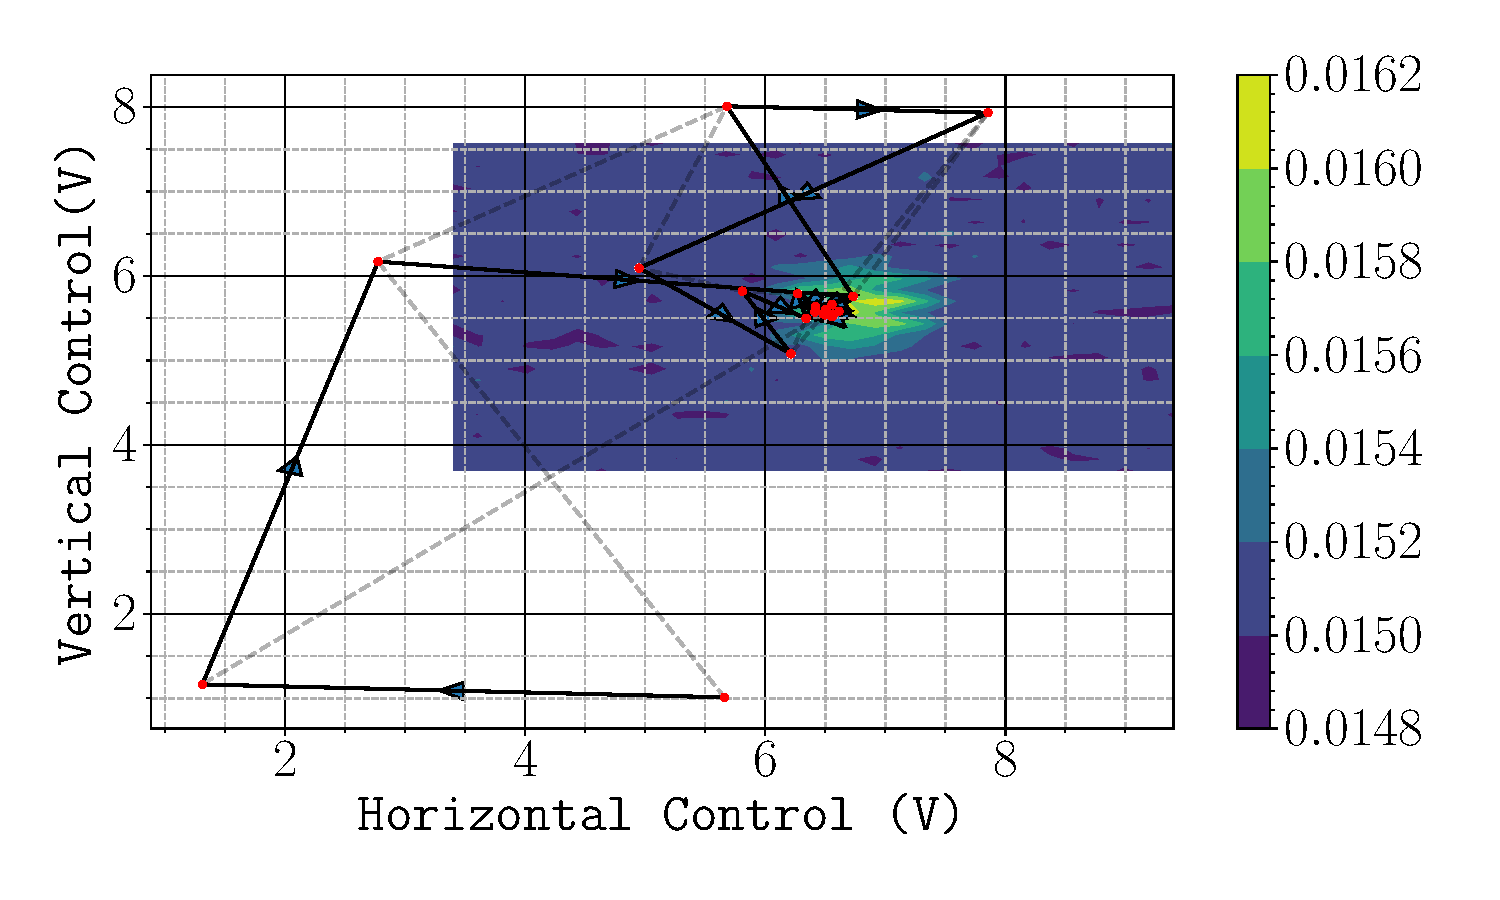
\includegraphics[width=0.5\textwidth]{simplex_alignment}
	\caption[Automatic mirror alignment using the Nelder-Mead simplex
		algorithm.]{Automatic mirror alignment using the Nelder-Mead simplex
		algorithm. This procedure starts by randomly selecting three pairs of
		control voltages for the horizontal and vertical piezo stacks. At each
		co-ordinate, the back-reflected power is measured. The algorithm proceeds by
		geometrically transforming the simplex using reflections, expansions and
		contractions, and updating the simplex using this new co-ordinate if the
		power measured is greater than the current lowest value. The algorithm uses
		the standard deviation of the last 5 values as a check for convergence. In
		this case, it terminates once the standard deviation is smaller than
		\sivalue{10}{\micro\volt}. The shaded lines indicate the simplex bounded by
		the three co-ordinates at each iteration, whose area reduces as the
		algorithm converges on the optimum value. A scan of the piezo control
		voltages close to the optimum is also plotted. The irregular shape of the
		measured power is a result of a hysteresis effect when the horizontal
		control voltage was changed from its maximum value to the minimum. Even with
		a low signal-to-noise ratio, the algorithm converged on a value close to the
		optimum. This resulted in a misalignment of less than
		\sivalue{13}{\micro\radian} along both axes.}
		\label{fig:simplex_optimisation} \end{figure}
\subsection{The Mechanical Accelerometer}\label{subsec:raman_mems}
The periodic interferometer signal means that the interferometer phase is only
proportional to acceleration over one fringe spacing \(\Delta a =
\frac{\pi}{\keff T^2}\). Furthermore, the fringe spacing is inversely
proportional to \(T^2\) so there is a trade-off between dynamic range and
sensitivity. These problems can be addressed by making use of a mechanical
accelerometer mounted onto the back of the retro-reflecting mirror to form a
hybrid system~\cite{Lautier2014}. The accelerometer determines the acceleration
up to the fringe spacing  and the interferometer measures the acceleration more
precisely. The accelerometer also measures the vibrations of the
retro-reflecting mirror, so it can be used to filter the effects of vibration
noise on the interferometer signal. This is discussed in more detail
in~\SectionRef{sec:vibration_senstivity}. This hybridisation scheme has been
used in measurements of gravity in high noise enivronments such as the centre of
Paris~\cite{Merlet2009} and in parablic aircraft
flights~\cite{Geiger2011a,Barrett2016a}. \par\noindent The accelerometer is a
navigation-grade AI-Q-2010 manufactured by \textit{Innalabs}. This particular
device was chosen because its specified intrinsic noise was
<\sivalue{7}{\micro\g} in the 0-100\ac{Hz} bandwidth. For a pulse separation \(T
= \sivalue{25}{\milli\second}\), the fringe spacing is
\(\sivalue{31.2}{\micro\g}\) so it is sensitive enough to measure the
acceleration to within one fringe. A schematic of this device is shown
in~\FigureRef{fig:innalabs}. It operates using a quartz pendulum which is is
free to move about one axis~\cite{Foote1992}. Under an acceleration, the
deflection of the pendulum is capacitively detected. A servo loop circuit drives
a current through the coils to restore the position of the pendulum. This
current is directly proportional to the acceleration of the pendulum. This model
has a nominal scale factor of \sivalue{1.235976}{\milli\ampere\per\g}. The
acceleration is measured using a load resistance of \sivalue{6}{\kilo\ohm} to
give an output voltage of \sivalue{7.56}{\volt\per\g}.
\begin{figure}[!htbp] \centering
	\resizebox{0.5\textwidth}{!}{\input{innalabs.pdf_tex}}
	\caption[Innalabs accelerometer cross-section]{Cross-section of the Innalabs
		AI-Q-2010 accelerometer.} \label{fig:innalabs}
\end{figure}
\subsubsection{Accelerometer Noise Spectrum}
\begin{itemize}
	\item Plot noise spectrum
	\item Explain how it differs when the table is floated
\end{itemize}
\section{The M-Squared Laser System}\label{sec:msquared_laser} \begin{itemize}
  \item M2 laser diagram \item Real-time communication \item Describe how it
  controls the frequency and phase of the two lasers \item DCS \end{itemize}
  This section describes the laser system manufactured by \textit{M-Squared
  Lasers}, which is used to drive Raman transitions. An overview of the laser
  system can be found in~\SectionRef{subsec:msquared_overview}, which includes
  the techniques used to externally communciate with the laser's ICE-BLOC
  control modules. The control of the frequency and phase-lock is then described
  in~\SectionRef{subsec:msquared_control}. Finally, this section concludes
  in~\SectionRef{dcs_module} with a description of the module used to control
  the output of the laser in real-time.
\subsection{Laser System Overview}
\label{subsec:msquared_overview} This system contains two Solstis lasers which
generate laser light by pumping a Ti-sapphire crystal housed inside a resonator.
The output light frequency is controlled using piezo-electric stacks to adjust
the resonator length. A schematic diagram of this laser system is given
in~\FigureRef{fig:msquared_laser}. Each laser is seeded using a
\textit{Lighthouse Photonics} Sprout laser to generate light around
\sivalue{780}{\nano\metre}. The first laser acts as the master whose frequency
is fixed. The second is slaved to this using a phase-locked loop to keep their
beat frequency and relative phase constant. The two beams are mxed on a
\ac{pbs}, so that they are orthogonally polarised. Two \acp{aoms} control the
output power. A planned upgrade for this system will have multiple outport ports
for the Raman light, which will require independent control. \par\noindent The
system contains 4 ICE-BLOC modules which implement various types of control. The
first two (one for each Solstis) are used to stabilise the output power of each
laser by feeding back to the corresponding Sprout laser. They are also used to
coarsely adjust the output frequency using a
\textit{HighFinesse} wavemeter. The third is used for the \ac{pll}
and feeds-back onto the slave laser to control both the frequency and phase of
the optical beat-note beteween the two lasers. The final ICE-BLOC, referred to
as the DCS module, is used to control the lasers in real-time during the
experiment.  \begin{figure}
	\centering \fontsize{10pt}{10pt}
	\resizebox{0.4\textwidth}{!}{\input{msquared_laser.pdf_tex}}
	\caption[M-Squared Laser System Schematic]{Schematic Diagram of the M-Squared
		laser system. Two Solstis lasers provide the two Raman frequencies, which
		are fibre coupled onto the orthogonal axes of a \ac{pm} fibre. Control of
		the power, frequency and phase as required to drive Raman transitions is
		handled by the four ICE-BLOC modules indicated in blue. Further detail of
		this control is given in the text.} \label{fig:msquared_laser}
\end{figure}

\subsubsection{External ICE-BLOC Control}
The ICE-BLOC modules are able to communicate with each other using an ethernet
hub. Another computer connected to this network is able to control them by
accessing a webpage that each module hosts. These webpages control the ICE-BLOCs
by sending structured JSON messages. This graphical interface can be bypassed by
directly communicating these messages. This is done using MOTMaster so that
various parameters, such as the frequency and phase of the Raman beat-note, can
be automatically varied between each experiment cycle. \subsection{Frequency and
Phase Control}\label{subsec:msquared_control}

\subsubsection{Master Lock}
The frequency of the master laser is stabilised using saturated absorption
spectroscopy in a rubidium vapour cell. Part of the beam is picked off and
modulated by an \ac{eom}. The positive frequency sideband is used to lock the
master laser to the 2,3 crossover feature. In effect, this means that the
modulation frequency of the \ac{eom} sets the one-photon detuning of the Raman
transition. The modulation frequency is set so that the master laser frequency
is \sivalue{1.13}{\giga\hertz} below the \trans{2}{3} transition.

\subsubsection{Frequency and Phase Lock} The optical beat-note between the two
lasers is measured using a fast photodiode. The signal from this is used in a
phase-locked loop to fix the relative phase between the two lasers. A frequency
divider halves the frequency of the signal before comparing it to a \ac{vco} of
around \sivalue{3.4}{\giga\hertz}. This creates an error signal which used to
control both the frequency and phase of the beat-note by feeding back to the
slave laser Solstis. The relative phase between the two lasers is adjusted using
an analogue phase shifter and the frequency difference is controlled by tuning
the \ac{vco} frequency. \par\noindent The beat-frequency of the Raman lasers can
be chirped by triggering a ramp of the control voltage to the \ac{vco}. For
chirp rates of lower than \sivalue{24}{\mega\hertz\per\second}, the phase-lock
is able to keep the beat-note phase-coherent during the chirp.  \subsection{The
DCS Module}\label{subsec:dcs_module} The DCS module is used to control the
output of the lasers during the experiment. It uses an on-board \ac{DDS} to
synthesise the \sivalue{80}{\mega\hertz} driving frequencies for each \ac{aom}.
The majority of the control is done using an \ac{fpga} that synthesises a timed
sequence of analogue and digital voltage waveforms. An example of a sequence
created using the DCS web interface is shown in~\FigureRef{fig:dcs_module}. The
sequence is segmented into individual steps and each channel can be separately
configured, much like the MOTMaster user interface. \par\noindent This module is
used to control the amplitude, frequency and phase of each Raman pulse. The
pulse amplitude is shaped using an analogue voltage to control the power of the
RF frequency. This has been calibrated so that the pulse can be shaped to
produce a square, Gaussian or Blackman amplitude envelope. A frequency chirp is
optionally triggered by sending a digital pulse to the \ac{pll} ICE-BLOC.
\par\noindent The synthesiser can be configured to run continuously, or to wait
at a chosen timestep for an external trigger. It can also iterate through a set
number of parameters, such as timestep duration or phase shift by re-building
the sequence after each cycle.  \begin{figure}[!htbp] \centering
	\resizebox{0.5\textwidth}{!}{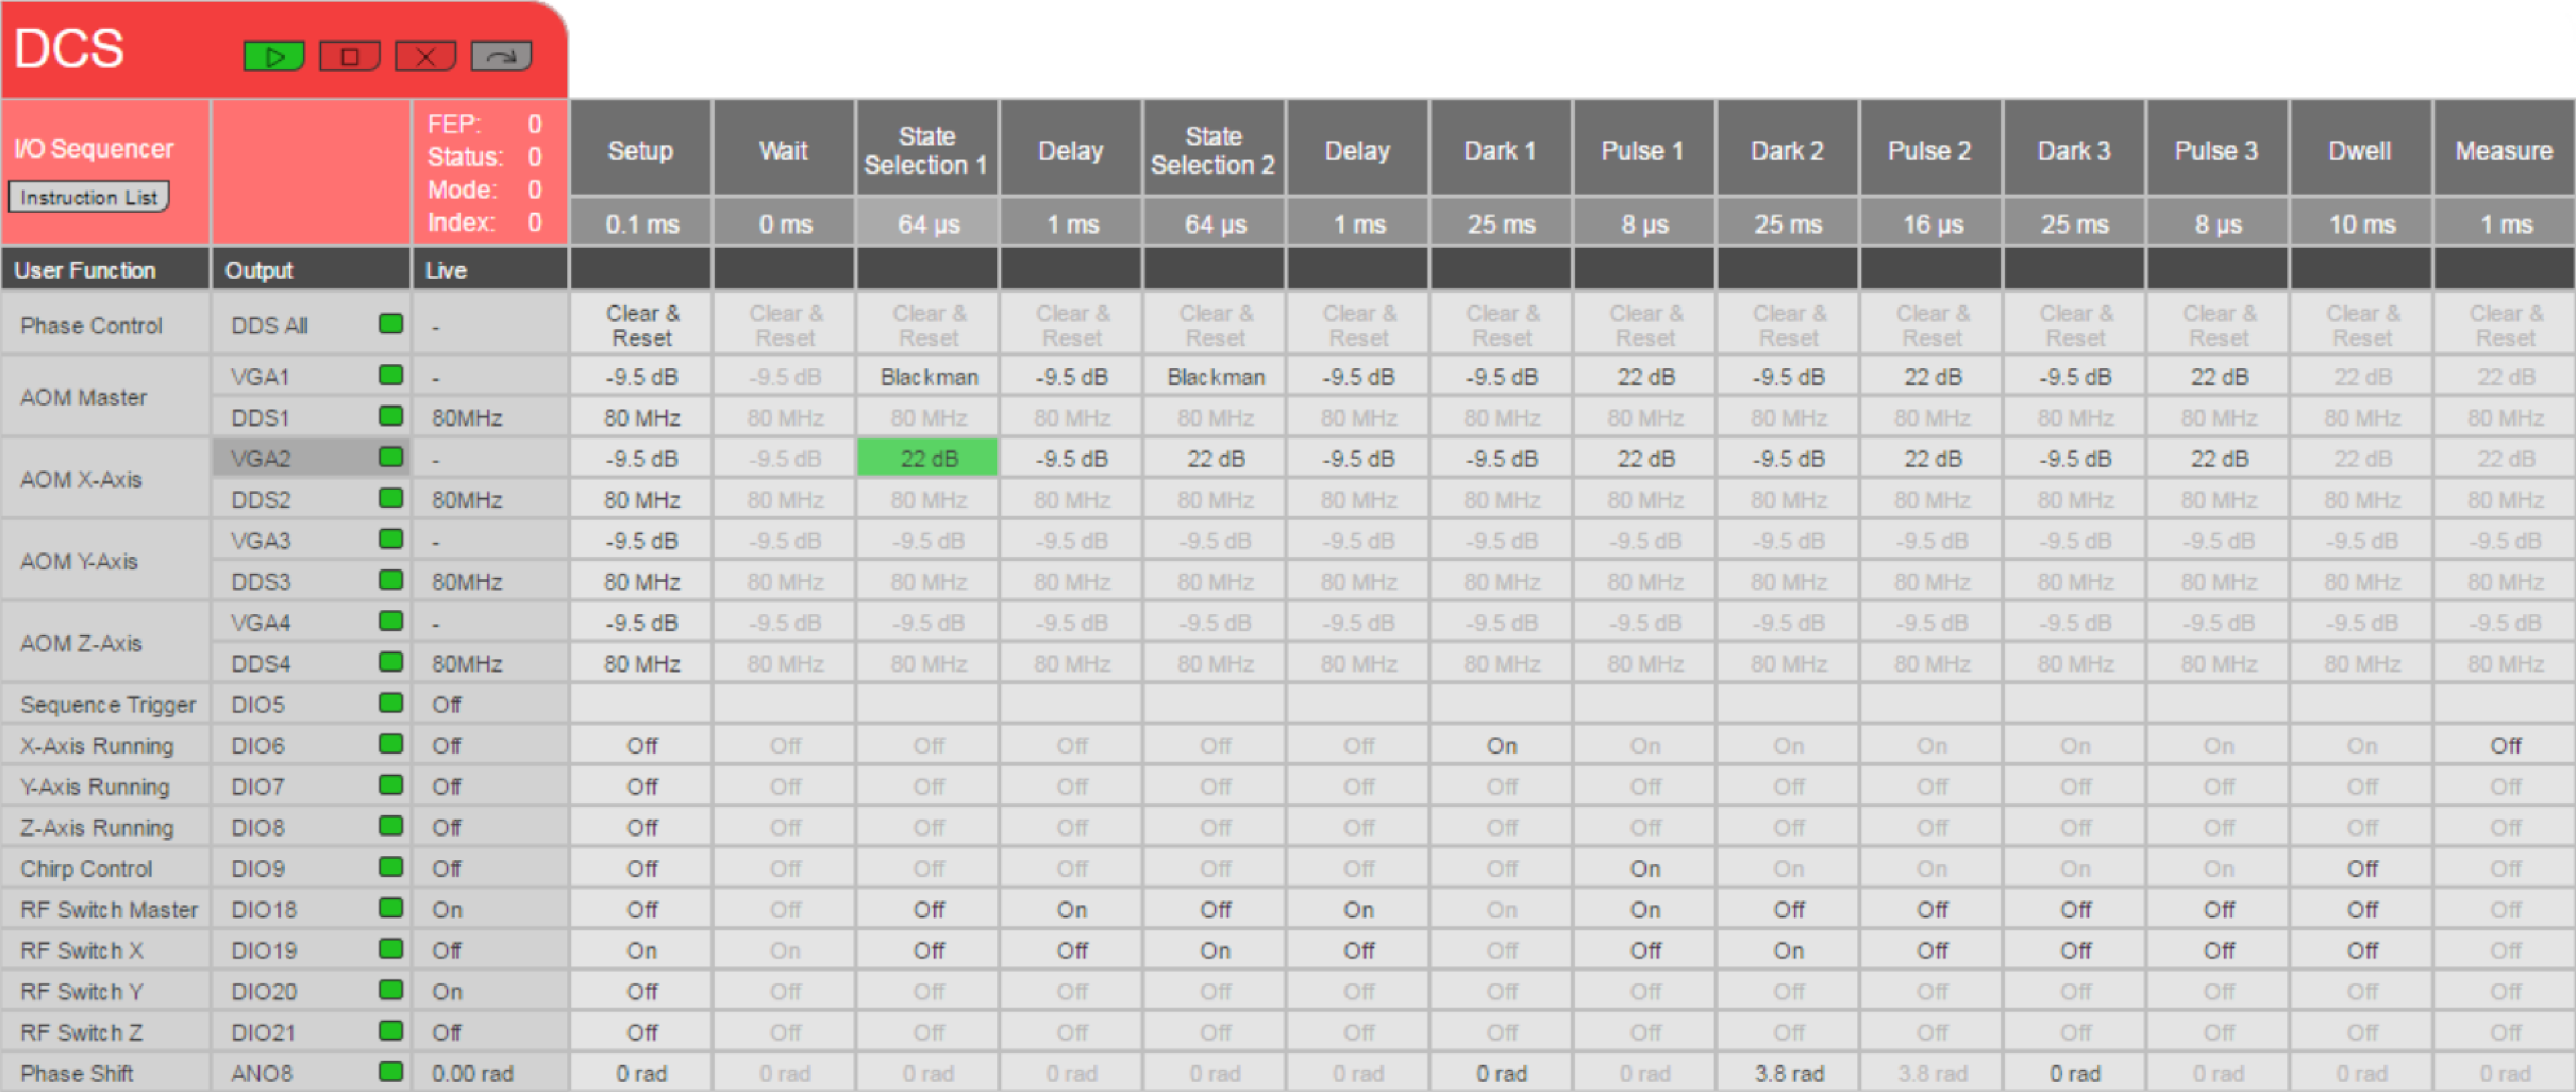
\includegraphics{dcs_module.pdf}}
	\caption[DCS Module User interface]{DCS module user interface. The sequence is
		synthesised from individual steps, The parameters of each Raman laser pulse
		can be configured independently.} \label{fig:dcs_module} \end{figure}
\section{Atom Detection}\label{sec:atom_detection} 
\begin{itemize} 
  \item Photodiode system - diagram 
  \item Detection sequence - diagram 
  \item Statistical analysis to estimate phase from measured voltages 
  \item Simulate detection curves?  
\end{itemize} 
This section describes the methods used to
measure the number of atoms in each hyperfine ground state. It begins with a
presentation of the other optical components used to detect the atoms by
driving \(\sigma^+\) transitions in~\SectionRef{subsec:photodiode_setup}.
The sequence of light pulses used to measure the number of atoms is then
given in~\SectionRef{subsec:detection_sequence}. This concludes with a
discussion on converting the measured photodiode signals into atom
number and interferometer phase.
\subsection{Optical Setup}\label{subsec:optical_setup}
A precise measurement of the number of atoms requires that the atom shot noise
is the dominant source of uncertainty in the measurement. The CCD used in
previous stages of the experiment is not sensitive enough for this as there is a
significant amount of noise in reading out the charge collected at each pixel.
Instead, a more sensitive photodiode is used to detect the atoms. With a
suitably high bandwidth, the readout time is much faster than the CCD as well,
so that the atoms can be detected well before they fall out of the field of
view. \par\noindent A diagram of the setup used to detect the atoms is given
in~\FigureRef{fig:photodiode_optics}. It is a triplet system which uses an
lenses with focal lengths \sivalue{150}{\milli\metre},
\sivalue{75}{\milli\metre} and \sivalue{60}{\milli\metre} in order from the
atoms to the photodiode.  A ray-tracing simulation of the optical system indicates spherical aberrations on the image. This is caused by the third lens, which was added to shorten the back focal length. The photodiode used is a \textit{Femto LCA-S-400K-SI},
which has a trans-impedence amplifier with a bandwidth of \sivalue{400}{\kilo\hertz} and a photo-sensitive area
with a diameter of \sivalue{3}{\milli\metre}. 
\subsubsection{Photodiode Calibration}
A calibration of the output voltage for an input collimated beam is
shown in~\FigureRef{fig:photodiode_calib}. This
gives a conversion factor of \sivalue{1.84e6}{\volt\per\watt}. 
\subsection{Detection using \(\sigma^+\) transitions}\label{subsec:photodiode_setup}
The atoms are detected using resonance fluorescence from two of the
circularly polarised \ac{mot} beams. A bias field polarises the atoms along the
\(\vec{z}\) axis, so that the light drives both \(\sigma^+\) and \(\sigma^-\)
transitions. Each Zeeman state has a different scattering rate, which
must be accounted for to calculate the number of atoms. This can be
simplified by flipping the handed-ness of
one of the \(\vec{z}\) \ac{mot} beams using a liquid-crystal
\ac{hwp}, so that both beams drive \(\sigma^+\) transitions. Now, the
atoms are optically pumped into \(\ket{2,2}\) and cycle on the
\(\ket{2,2} \rightarrow \ket{3,3}\) transition. Only this scattering
rate is required to determine the number of atoms.
\par\noindent
\FigureRef{fig:detection_scheme} shows the setup used to invert the
polarisation of one \ac{mot} beam for detection. The liquid-crystal waveplate is an electro-optical device whose birefringence changes when an ac voltage is applied across it. The waveplate is placed at the output of the downward-propagating (\(\vec{z}_-\))
collimator. 
  \begin{figure}[!htpb]
    \centering
    %    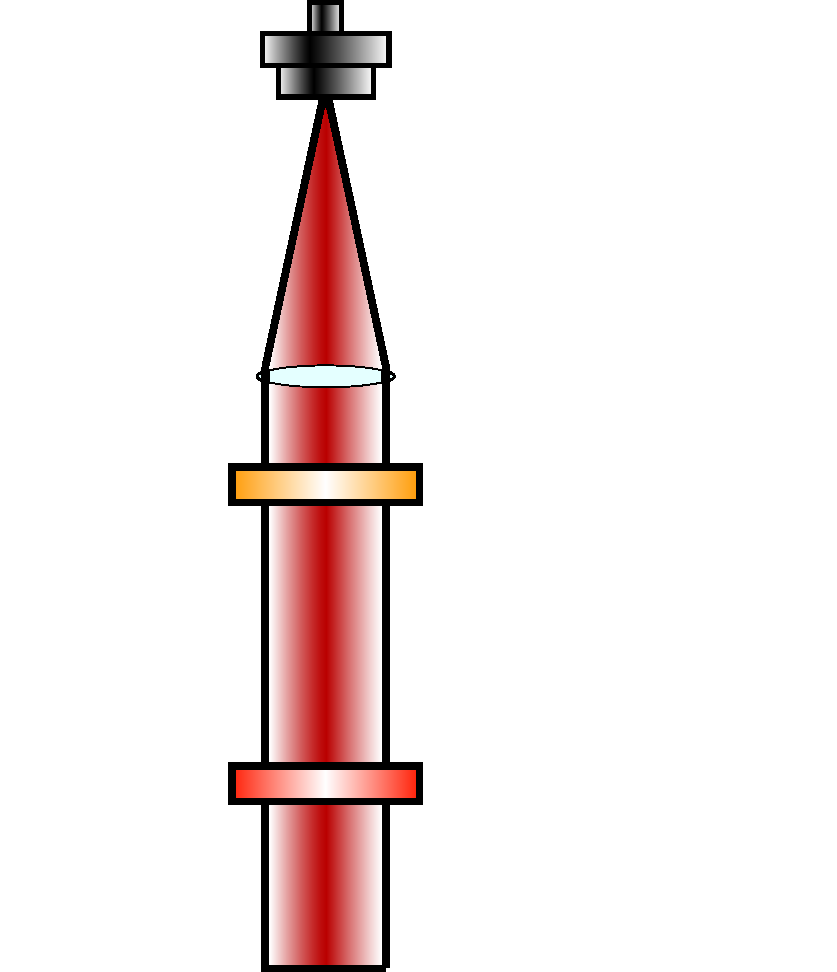
\includegraphics{detection_scheme.pdf}
    \caption{Scheme for detection by driving \(\sigma^+\) transitions. A
      liquid-crystal waveplate flips the handedness of the \(\vec{z}_-\) \ac{mot} beam. The atoms then fluoresce on the \(\ket{2,2} \rightarrow \ket{4,3}\) cycling tansition}\label{fig:detection_scheme}
\end{figure}
\begin{figure}[!htbp] 
  \centering \fontsize{18pt}{18pt}
	\resizebox{0.7\textwidth}{!}{\input{photodiode_optics.pdf_tex}}
	\caption[Optical setup for Photodiode Detection]{Optical setup for photodiode
		detection. A triplet lens system focuses light from radiated from the atoms
		onto a photodiode. This is mounted using a translation stage to
  position the photodiode at the back focal point.}
  \label{fig:photodiode_optics}
\end{figure}
\subsubsection{Detection Sequence}\label{subsec:detection_sequence}
detection volume for a longer period of time. The intensity of the
light is reduced to around \(I_\text{sat}\), so that the
scattering rate per atom is approximately linear. The photodiode is
triggered to start at the first Dwell time. The cooling light is first
switched on, so that only atoms in \(\ket{F=2}\) scatter light. After this, the repump
is switched on, so that atoms in \(\ket{F=1}\) are optically pumped
into \(\ket{F=2}\) and all the atoms scatter light. This repump light is a
sideband of the cooling laser, so the total output is increased
to ensure that the intensity of the cooling light remains constant.
Each detection step lasts \sivalue{250}{\micro\second}, but the
first \sivalue{50}{\micro\second} is discarded to allow time for the
intensity to stabilise and for optical pumping into \(\ket{F=2}\).
The atoms are then blown away by switching off one of the detection
beams before the sequence is repeated to collect a
background signal.
\begin{figure}[!htbp] 
  \centering
  \resizebox{0.7\textwidth}{!}{\input{detection.pdf_tex}} 
  \caption[State detection sequence timing]{Timing diagram for state
  detection. Atoms in \(\ket{F=2}\) are detected before the repump
light pumps those in \(\ket{F=1}\), so they are detected as well. A
background light measurement for each step is also taken.}
	\label{fig:detection} 
\end{figure} 
\subsection{Measuring the Occupation Probability}\label{subsec:phase_measurement}
The occupation probability is obtained by measuring the proportion of
atoms in each hyperfine ground state. The number of atoms
\(n_\text{at}\) that scatter light on the cycling transition is
proprtional to the photodiode voltage \(U_\text{pd}\) as follows
\begin{equation}
  U_\textnormal{pd} &= \eta R_\text{sc}(I,\Delta) n_\text{at} \hbar \omega G \nonumber \\
  &= \alpha \eta R_\text{sc}(I, \Delta) n_\text{at}
  \label{eq:pd_signal}
\end{equation}
where \(\eta = \Omega/4\pi\) is the fractional solid angle subtended by the
collection optics, \(\hbar\omega = \sivalue{1.6}{\electronvolt}\) is
the photon energy, \(R_\text{sc}\) is the scattering rate defined
in~\EquationRef{eq:scattering_rate} and \(G\) is the photodiode
conversion gain. The probability of an atom occupying \(\ket{F=2}\) is calculated
as follows
\begin{equation}
  \text{P}_{\ket{F=2}} =
  \frac{\text{N}_2-\text{B}_2}{\text{N}_\text{Tot} -
  \text{B}_\text{Tot}}
  \label{eq:prob_measurement}
\end{equation}
where N and B denote the signal and background measurements,
respectively. Subtracting the background signal from each measurement
removes the bias that arises from detecting light not
scattered by the atoms. Under a constant scattering rate and
collection efficiency, the scaling factor between atom number and
photodiode voltage cancels in~\EquationRef{eq:prob_measurement}. The interferometer phase \(\Phi\) is
determined from \EquationRef{eq:prob_measurement} using
\begin{equation}
\text{P}_{\ket{F=2}} = \text{P}_0 +\frac{C}{2}\cos(\Phi/2)^2
  \label{eq:interferometer_phase}
\end{equation}
where 
\subsection{Sources of Detection Noise}\label{subsec:detection_noise}
\begin{itemize}
  \item Contributions to detection noise
  \item Calibrating detector
  \item Atom-equivalent noise
\end{itemize}

Each measurement of the number of atoms has a systematic uncertainty due to
random processes that influence the detection signal. This error
propagates to given an uncertainty and the interferoemter phase and
hence, acceleration. Characterisation of these noise sources is
required to understand their effects on the sensitivity to
acclerations.
These both have shot noise fluctuations which introduce an uncertainty
on the interferometer phase. Finally, there is also technical
noise in the detector itself. The contribution from each source can be
understood using their power spectral densities. 
\subsubsection{Atom and Photon Shot Noise}
The discrete nature and the fact that atoms are loaded into the
experiment and scatter photons at a constant rate mean that the
statistics on the number of atoms and photons are well-described by
Poission distributions. Therefore, the number of atoms in the
interferometer and number of photons arriving at the detector have
shot noise fluctations with variances given by their mean values. From~\EquationRef{eq:pd_signal}, these are related to an
equivalent output voltage as follows
\begin{align}
  \sigma_\text{at,v}^2 &= \alpha^2 \eta^2 R_\text{sc}^2 n_\text{at}\\
  \sigma_\text{p,v}^2 &= \alpha^2 \eta R_\text{sc} n_\text{at} 
  \label{eq:atom_photon_noise}
\end{align}
where \(\sigma_\text{at,v}\) dominates, provided at least one photon
per atom is detected. For a large number of particles, shot noise
approaches a Gaussian distribution, which has a uniform power spectral
density. However, the finite detection time acts as a low-pass filter by limiting
the influence of frequency components above the sampling frequency.
In the time domain, the signal is convolved with a rectangular pulse
of a characteristic time \(\tau\), so the power spectral density is a
product of the individual power spectral densities
\begin{equation}
  S(f) = 2 S_0\left(\frac{\sin(\pi f \tau)}{\pi f \tau}\right)^2
  \label{eq:psd_shot_conf}
\end{equation}
where \(S_0\) is the one-sided power spectral density of the shot
noise component. From the Wiener-Khinchin theorem, the variance is
equal to the integral of the power spectral density, so
\begin{equation}
  S_0 = \sigma^2_\text{i,v} \tau
  \label{eq:shot_noise_amp}
\end{equation}
For shorter detection times, this has the effect of aliasing
high-frequency noise into the lower-frequency components.  
%The number of photons
%arriving at the detector in a time interval \(\Delta t\) is given by
%\begin{align}
%  n_p &= N R_\text{sc}(I,\Delta) \eta \delta t \nonumber\\
%  &= \alpha N
%  \label{eq:photon_detector}
%\end{align}
%where \(\eta\) is the collection effiency of the detector, \(N\) is
%the number of atoms and \(R_\text{sc}\) is the scattering rate defined
%in \EquationRef{eq:scattering_rate}. The atom shot noise and photon
%shot noise are given by \(\sigma_N = \sqrt{N}\) and \(\sigma_p =
%\sqrt{n_p}\), respectively. The
%uncertainty in the number of detected photons \(\sigma_D\) has
%contibutions from both the atom shot noise and the photon shot noise
%\begin{equation}
%  \sigma_D = \sqrt{\alpha^2\sigma_N^2 + \sigma_p^2} 
%  \label{eq:detection_uncertainty}
%\end{equation}
%This is dominated by the atom shot noise when \(\alpha^2 > 1\), i.e. when
%more than one photon per atom is detected by the photodiode. 
%\par\noindent
%There is additional contribution to \(\sigma_D\) from the technical
%noise of the detector. The signal from the photodiode is averaged over
%the detection time \(\Delta t\), so the variance in this is given by
%\begin{equation}
%  \sigma_v = \int_0^{f_c} |S_\text{pd}|^2 \mathrm{d}f 
%  \label{eq:photodiode_noise_bandwidth}
%\end{equation}
%where \(|S_\text{pd}|^2\) is the one-sided power spectral density of the
%photodiode signal and \(f_c = 1/(2\Delta t)\) is the frequency
%bandwidth.   
\subsubsection{Photodiode Technical Noise}
A further source of noise is technical noise in the photodiode and
amplifier. This
arises from multiple electronic processes -- such as Johnson noise and shot noise in
the current -- but it is not necessary to consider them independently
in the following discussion. Since this technical noise does not
depend on the number of atoms, it adds a systematic uncertainty to the
measured interferometer phase. 
The technical noise of the photodiode and amplifier is a source of
uncertainty in the output voltage. The \ac{nep} is
useful in determining the noise from the photodiode when the signal is
averaged over a given integration time. A plot of the noise-equivalent
power of the photodiode is shown in~\FigureRef{fig:photodiode_nep} taken
with a sampling frequency of \sivalue{200}{\kilo\hertz}. The
photodiode was covered and the output voltage was sampled for
\sivalue{2}{\second}. The power sp has been calculated
using Welch's method~\cite{Welch1967}. This partitions the data before
calculating the Fourier transform of each subset and taking the
average. This has the effect of reducing the variance in the estimated
power spectrum at the expense of reducing the frequency resolution.
The \ac{nep} is then given by
\begin{equation}
  NP(f) = \frac{1}{G R } S(f)
  \label{eg:nep_psd}
\end{equation}
where \(G = \sivalue{1e7}{\volt\per\ampere}\) is the transimpedence Gain,
\(R = \sivalue{0.54}{\ampere\per\watt}\) is the reponsivity of the
photodiode and \(S\) is the amplitude spectral density.

\begin{figure}[htpb!]
  \centering
  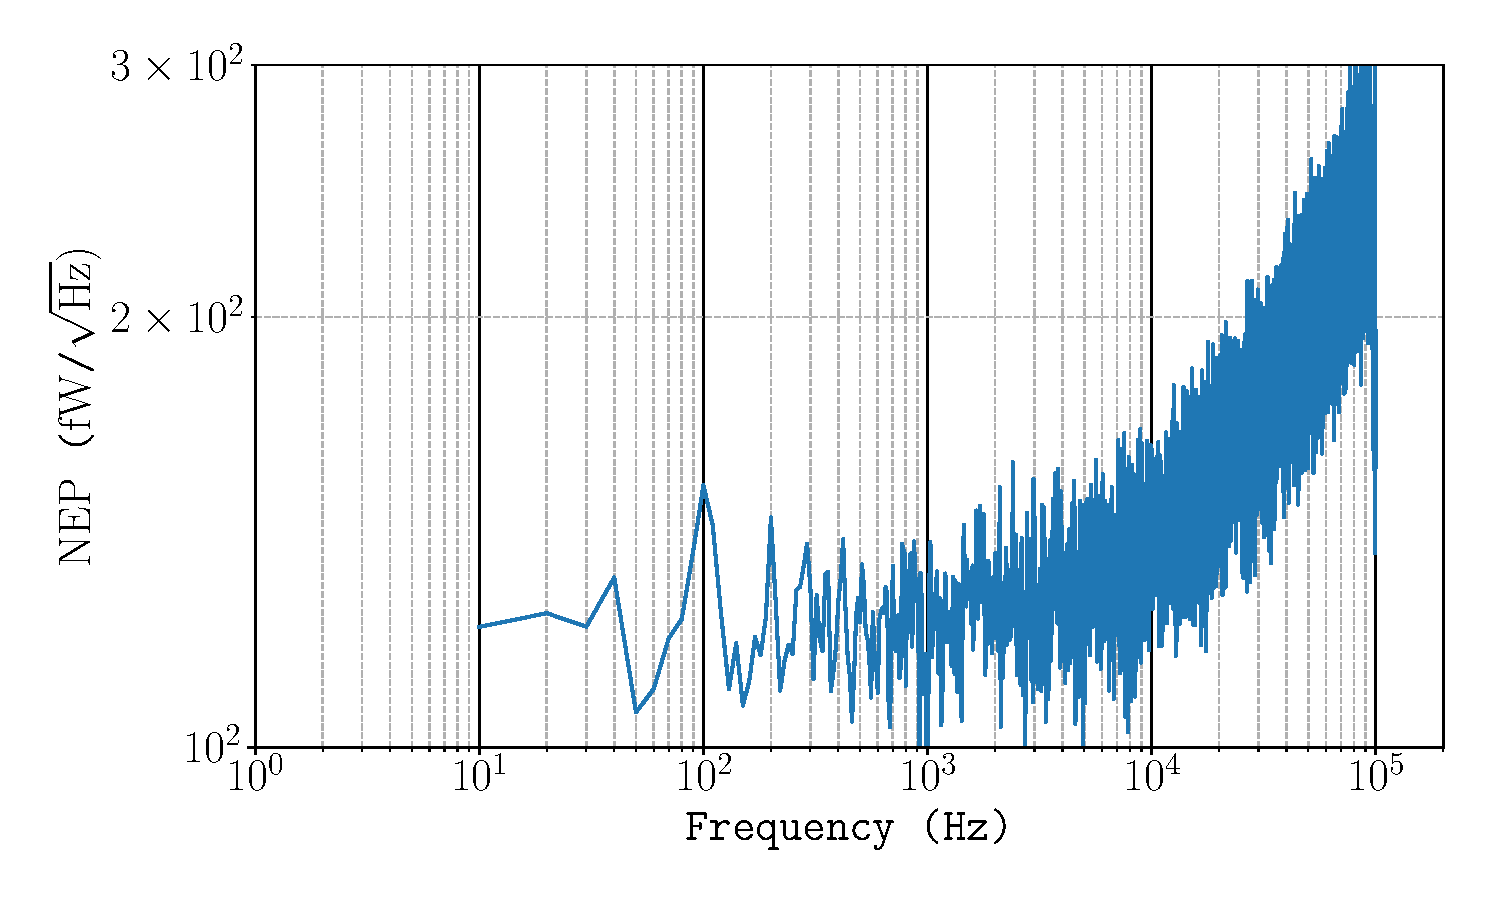
\includegraphics{pd_psd}
  \caption[Power spectral density]{Power spectral density of the photodiode output voltage
  sampled for \sivalue{2}{\second} at a rate of \sivalue{\kilo\hertz}.}
  \label{fig:pd_psd}
\end{figure}
\section{Individual Pulse Characterisation} \label{sec:atomint_rabiosc}
\subsection{Raman Spectrum}
\begin{itemize}
	\item Raman transition spectrum identifiying Doppler width
	\item Explain the large co-propagating peak
	\item Asymmetry between \(\pm k\)
\end{itemize}
\subsection{Velocity-Selective Pulse}
\begin{itemize}
	\item Spectrum after velocity selection
	\item How does linewidth of Raman pulse affect final velocity distribution?
	\item Why do we need this?
	\item Final Doppler width
\end{itemize}
\subsection{Interferometer Pulses}
\begin{itemize}
	\item Pulse characterisation for each pulse
	\item Fit to dephasing
\end{itemize}

\section{Three-Pulse Atom Interference} \label{sec:atomint_threepulse}
\subsection{Fringe Contrast vs. Launch Trajectory}\label{subsec:launch_contrast}
\section{Measuring Accelerations}\label{sec:atomint_accelerations}
\subsection{Vibration Sensitivity}\label{sec:vibration_senstivity}
The mirror defines an inertial frame of reference -- the interferometer measures
acceleration of the atoms relative to the acceleration of the mirror. Vibrations
of the mirror introduce a component of the interferometer phase which is
independent of acceleration. This vibration-induced phase can be accounted for
by mounting the accelerometer onto the back of the mirror. During the
interferometer, the accelerometer measures the acceleration of the mirror.

\section{Sensitivity}
\subsection{Loading Rate}
A fundamental limit to the uncertainty on the number of atoms is given by the
statistics of the total number of atoms in the experiment. For short loading
times, atoms are loaded into the \ac{mot} at a constant rate, so the total
number of atoms after the experiment follows a Poisson dis 
\subsection{Detection Noise}
The
\subsection{Vibrations}









